\documentclass[12pt]{article}

\usepackage[ruled,vlined,linesnumbered]{algorithm2e}
\usepackage{graphicx}
\usepackage{times}
\usepackage{anysize}
\usepackage{hyperref}
\marginsize{2cm}{2cm}{2cm}{3cm}
%\onehalfspace
%\doublespace
\setlength{\parindent}{0.8cm}
%\setlength{\parskip}{0.2\baselineskip}
%\setlength{\topmargin}{2cm}
%\setlength{\textheight}{25cm}
%\setlength{\textwidth}{14cm}
%\setlength{\oddsidemargin}{2cm}
%\setlength{\evensidemargin}{2cm}
\usepackage{fancyhdr}
\pagestyle{fancy}
\setlength{\headheight}{14.5pt} 

\newcommand{\note}[1]{\textbf{\textit{#1}}}
%\newcommand{\note}[1]{}
\newcommand{\astar}{A$^*$}
\newcommand{\tuple}[1]{\ensuremath{\left \langle #1 \right \rangle }}
\newcommand{\eff}{\textit{eff}}
\newcommand{\pre}{\textit{pre}}

\newtheorem{theorem}{Theorem}
\newtheorem{observation}{Observation}
\newtheorem{corollary}{Corollary}

\newtheorem{problem}{Project Goal}

\linespread{1}

\lhead{Data-and-Model Driven Reasoning} \rhead{B. Juba and R. Stern}
\cfoot{\thepage} 
%\cfoot{} 
\pagenumbering{arabic}
%\pagenumbering{Roman}

\begin{document}

%\title{Learning Common Sense Rules Multi-Agent Reasoning with Common}
%\title{Augmenting Model-based Approaches for Diagnosis, Planning, and Plan Recognition with Data}
%\title{Diagnosis, Planning, and Plan Recognition with An Approximate Model and an Abundance of Data}
\title{Data-and-Model Driven Reasoning}
%\note{Need to shorten to 250 words}

\begin{center}
\LARGE{Research Plan}
\end{center}

\section{Scientific and Technological Background}
% 1. From BSF guidelines: A brief description of the subject and the scientific and technological background;


% Planning and diagnosis are important, and prior work mostly used a model-based approach
Automated planning and automated diagnosis (DX) are long term goals of Artificial Intelligence (AI) research, with many practical applications~\cite{abreu2011simultaneousDebugging,fox2011automatic,niggemann10model,williams96,robinson2014cost,ruml2011line,Zamir2014UsingMD}. Traditional algorithms for planning and for diagnosis employ {\em model-based reasoning}: an underlying model of the world is assumed and is used to generate plans or infer diagnoses. Classical STRIPS planning~\cite{fikes1971strips} is a prime example of model-based planning: the world model is a collection of first-order predicate calculus formulas that describe states, actions' preconditions and effects, and relevant ``frame axioms''~\cite{ghallab2004automated}. In model-based diagnosis (MBD) the world model describes the behavior of the diagnosed system, 
possibly also as a set of first-order formulas~\cite{reiter1987theory,deKleer1987diagnosing}. 
%[[Roni: maybe this is better]] In consistency-based diagnosis, the world model describes the behavior of the diagnosed system, possibly also as a set of first-order, and diagnoses are assumptions consistent with this model and observations.



% Data-driven is an alternative approach to model-based
Data-driven methods have been proposed as an alternative approach to model-based reasoning for performing many AI tasks. %, including planning and diagnosis. 
Instead of having a world model, data-driven methods  assume that the world is observed and these observations are given as input. Then, Machine Learning (ML) algorithms are used to learn a model that approximates the world, in a way that allows us to perform model-based reasoning effectively. Some data-driven approaches even directly learn how to act/diagnose/reason without generating a model of the world (e.g.,~\cite{kearns2002POMDPsample}). 
With the growing availability of data and computing power, much of the current AI efforts are data-driven,
and data-driven algorithms have been proposed for  planning~\cite{fern2011first,juba2016jmlr} and diagnosis~\cite{keren2011model,qin2012survey}.


% Both approaches have pros and cons
Both approaches -- model-based and data-driven --  have pros and cons, and each use different algorithmic tools (logic and decision theory vs. statistics and ML) and consider different sources of information (model vs. past observations). Data-driven methods overcome an inherent obstacle in model-based reasoning -- the need for an accurate enough model of the environment. Moreover, Valiant argues that  data-driven mechanisms also compensate for the kind of errors that are introduced as a result of  reasoning with a model that is an approximate representation of the world~\cite{valiant2000neuroidal,valiant2000robustLogics}.
%Valiant argues that in addition to naturally solving the problem of large-scale knowledge acquisition, data-driven mechanisms also compensate for the kind of errors that are introduced as a result of  reasoning with a model that is an approximate representation of the world~\cite{valiant2000neuroidal,valiant2000robustLogics}.
However, unless similar situations were observed in the past, data-driven methods do not provide correctness guarantees (for the generated plan or the found diagnosis)  
while model-based reasoning provide a principled,  well-studied approach to reason about every situation in which the model holds. %generate new plans and diagnoses. % about novel . %generate plans or diagnoses that are provably correct even in situations that were not observed before. 

% Provable correctness is limited in scope. Covers all possible cases, data-driven onlya pplicable to what was observed. Principled looses...


% We will show how to use both model and data
%[[Roni: Previous version]]
%We propose to {\bf develop an integrated data-and-model driven approach for solving planning problems and for solving diagnosis problems that use available observations and world models.} The proposed research includes laying theoretical foundations for this data-and-model driven approach as well as developing concrete planning algorithms and diagnosis algorithms that outperform the current state-of-the-art, which usually use either a model-based or a data-driven approach. The key novelty in the proposed research is not in the use of model and past observations, but in  the synergy of the algorithmic ideas from the data-driven and model-based literature. 
 


%\note{Need to improve the paragraph below: make things more concerete: what are model and observations in planning and in diangosis, what are our approaches?}
%We will cover a broad range of settings, from having a complete model of the relevant world with a limited  number of observations, to having a large set of observations and a partial and uncertain world model. When a complete model is available, we will explore how data-driven methods can exploit given observations to speed up model-based reasoning and improve the quality of the solution found. When only an incomplete and possibly inaccurate model is available, data-driven methods have a larger role, using available observations also as means for better understanding the real world dynamics. To this end, we will build on PAC semantics, an elegant and theoretically sound framework to learn rules of the environment dynamics that are correct in most cases with high likelihood (hence the name, ``{\underline P}robably {\underline A}pproximately {\underline C}orrect''). PAC semantics also provide a natural way to integrate rules that are learned from observations and rules that are part of a given world model, where the latter will be additional PAC-semantic rules having high confidence. Nonetheless, with the exception of PI Juba's preliminary work~\cite{juba2016jmlr,juba2016aaai,zhang2017aaai}, there has been no work on using PAC semantics for planning or diagnosis. We outline below the challenges in doing so and how we aim to address them. [[Roni: End of previous version]]
%, as there are unique challenges in doing so. 



%[[Roni: New version]]
We propose to {\bf develop an integrated data-and-model driven approach for solving planning problems and diagnosis problems that use available observations and world models.} The key novelty in the proposed research is the use of PAC semantics~\cite{valiant2000robustLogics}, 
an elegant and theoretically sound framework to learn rules of the environment dynamics that are correct in most cases with high likelihood (hence the name, ``{\underline P}robably {\underline A}pproximately {\underline C}orrect''). PAC semantics provides a natural way to integrate rules that are learned from observations and rules that are part of a given world model, where the latter will be additional PAC semantic rules having high confidence. Moreover, the PAC-semantics framework allows reasoning about the relation between the number of observations available and the usefulness of the information learned, thus providing guidelines for when additional observations are needed. 
Nonetheless, with the exception of PI Juba's preliminary work~\cite{juba2016jmlr,juba2016aaai,zhang2017aaai}, there has been no work on using PAC semantics for planning or diagnosis. We outline below the challenges involved and how we aim to address them. 


The proposed research includes laying theoretical foundations for the proposed data-and-model driven approach as well as developing concrete planning algorithms and diagnosis algorithms. We expect these algorithms to outperform the current state-of-the-art, which usually use either a model-based or a data-driven approach, in addition to having 
%\note{Need to improve the paragraph below: make things more concerete: what are model and observations in planning and in diangosis, what are our approaches?}
The proposed research will consider a broad range of settings, from having a complete model of the relevant world with a limited  number of observations, to having a large set of observations and a partial and uncertain world model. When a complete model is available, we will explore how data-driven methods can exploit given observations to speed up model-based reasoning and improve the quality of the solution found. 
When only an incomplete and possibly inaccurate model is available, data-driven methods have a larger role, using available observations also as means for better understanding the real world dynamics. Using PAC semantics in each of these settings is challenging. We outline below these challenges and how we aim to address them. 
%[[Roni: End of new version]]



% We are awsome for this
This project directly builds on the individual expertise of each PI. Most of PI Juba's work has been on data-driven mechanisms, while most of PI Stern's work has been on model-based algorithms for planning and for diagnosis. Moreover, both PIs have independently started to work on how to combine model-based and data-driven methods specifically for planning and for diagnosis: PI Juba's work laid theoretical foundations for such a combination~\cite{juba2016aaai,juba2016jmlr} while PI Stern's proposed practical planning and diagnosis algorithms that effectively use both models and observations~\cite{elmishali2016dataAugmented,stern2011probably,stern2012search}. 
Recently, the PIs collaborated in initial work on using PAC semantics in planning~\cite{stern2017efficientAndSafe}. 
The results are encouraging, but are currently limited to a very specific setting: classical planning, where only normal trajectories are observed, 
and there is no a-priori knowledge of the domain. 
This research project is intended to extend well beyond this initial work, providing planning and diagnosis algorithms 
that are robust and applicable in a range of settings, and have a strong theoretical foundation. 
%Developing this preliminary work further to broader settings and to diagnosis  requires di
%[[Mention joint work in IJCAI?]]
 
 %you can phrase it better - This project directly builds on the individual expertise of each PI... You should add a sentence about the achievements of each that shows they are an expert, e.g. a first algorithm to be deployed in a given setting, 
 

\section{Objectives and Significance}
%2. From BSF guidelines: Objectives and significance of the research

%The first setting we will study is where an accurate model of the world dynamics is given along with a set of observations. In this setting we will pursue the following concrete set of objectives. 
We propose to pursue the following concrete set of objectives:
% PAC semantics is cool, but they have not been used for serious reasoning tasks :)
\vspace{-0.35cm}

\paragraph{Objective \#1. Data-and-model driven planning with PAC-semantic rules.}
%\paragraph{Objective \#1. Learning and using PAC-semantic rules for planning} 
%\paragraph{Objective \#2. Data-driven learning of PAC semantic rules for model-based planning.}
PAC semantics have been applied to classical learning tasks such as prediction of missing words in text~\cite{michael2008first} and user profiling in a recommender system~\cite{semeraro2009knowledge}. Planning is a fundamentally different type of reasoning task in that it is inherently about causal relationships over a changing distribution. Key questions arise, such as how to identify which state variables are preconditions of an observed action, and how to identify rules that are effective for planning. We will address these fundamental questions, and 
develop effective algorithms that plan with PAC semantic rules. PI Juba has started to explore the challenges raised when learning and using PAC semantics for planning, and these initial results suggest that integrating learning into planning simplifies both tasks~\cite{juba2016jmlr}. Preliminary joint work by the PIs suggested on classical planning explored how such rules can be learned and used instead of a world model~\cite{stern2017efficientAndSafe}. 

%We will explore the relation between planning with PAC semantic rules and other planning formalisms, and in particular consider adapting existing planning algorithms for this purpose. The initial work by PI Juba suggests that integrating learning into planning simplifies both tasks~\cite{juba2016jmlr}. 

\vspace{-0.35cm}
%\paragraph{Objective \#1. Learning and exploiting the relation between planning heuristics and actual cost.}
\paragraph{Objective \#2. Model-based planning with data-driven PAC heuristic search.}
Model-based planning often uses heuristic search. We will explore ways in which data-driven methods can be used to learn from past observations (executed plans) the probabilistic relationship between planning heuristics and the costs they estimate. Then, we will explore how knowledge of this relationship can be used to improve search-based planning algorithms, following prior work by PI Stern~\cite{stern2011probably,stern2012exploring,stern2014potential}.
%We will explore how to learn from past trajectories (plans) the probabilistic relation between planning heuristics and the costs they estimate. Given such knowledge, we will develop planning algorithms that exploit this knowledge. Prior work by PI Stern has demonstrated the potential of such approaches~\cite{stern2011probably,stern2012exploring,stern2014potential}. % but major challenges are ...
That prior work left many fundamental research questions open, such as: What assumptions are needed to properly generalize from past observations to future planning sessions? What are the theoretical guarantees one can achieve with these observations? And, how many observations are needed to effectively assist the planner? Answering these questions has driven part of this collaboration with PI Juba, who is an expert in learning theory. 



%. 

%\note{Maybe we should merge objectives 2 and 3}
%\paragraph{Objective \#3. Data-and-model driven planning with PAC semantic rules.}
%In addition to learning a set of PAC semantic rules for planning, we will develop effective planning algorithms that use these rules. We will explore the relation between planning with PAC semantic rules and other planning formalisms, and in particular consider adapting existing planning algorithms for this purpose. The initial work by PI Juba suggests that integrating learning into planning simplifies both tasks~\cite{juba2016jmlr}. 
%PI Juba has started to explore the challenges raised when using PAC semantics for planning~\cite{juba2016jmlr}. 

\vspace{-0.35cm}
\paragraph{Objective \#3. Augmenting MBD algorithms with data-driven fault-prediction models.} 
We propose to learn a {\em fault prediction model} from observations, and then explore how such a learned fault predictor can augment existing MBD algorithms. 
One particularly attractive direction we will pursue is to use these predictions as a means to bias MBD algorithms towards finding diagnoses that are more likely to be true. This is sorely needed as MBD algorithms are known to return an overwhelmingly large number of possible diagnoses~\cite{stern2015many}. Being able to identify the more likely diagnoses will allow more accurate diagnoses and more informed decision making. PI Stern's initial results on this data-augmented approach for diagnosis are promising~\cite{elmishali2016dataAugmented}. But, a more rigorous theoretical foundation is needed to enable us to answer key questions such as how many observations are needed to effectively improve diagnosis accuracy, what is required to enable the prediction of future faults using past observations, and whether or not we can transfer this knowledge to other, similar systems. Again, the collaboration between the PIs is especially suitable to answer these questions. 

%what assumptions are needed to properly generalize from past observations to future planning sessions? what are the theoretical guarantees one can achieve with these observations? and how many observations are needed to effectively assist the planner? Answering these questions is exactly what has driven the collaboration with PI Juba, which is an expert in learning theory.



% Challenges
%\note{TODO: Distribute this paragraph throughout this section}While the preliminary results of PI Stern for the two objectives above are encouraging, they give rise to several fundamental research questions: what assumptions are needed to properly generalize from past observations to future reasoning? what are the theoretical guarantees one can achieve with these observations? and how many observations are needed to effectively assist the reasoning process? Answering these questions is exactly what has driven the collaboration with PI Juba, which is an expert in learning theory. 

\vspace{-0.35cm}
\paragraph{Objective \#4. Data-and-model driven diagnosis with PAC-semantic rules.} 
%\paragraph{Objective \#4. Learning and using PAC-semantic rules for automated diagnosis} 
As with planning, we will develop algorithms to learn 
relevant PAC-semantic rules from observations and develop diagnosis algorithms that use these rules. There are few attempts to perform model-based reasoning with approximately correct models, and thus we expect the resulting MBD algorithms to have a substantial impact on practitioners and researchers.  



%[[From e-mails]] For our own work, even if we can't nail down precisely when our algorithms work well, we will still strive to obtain some partial understanding of when and why the approach works, as is being done for SAT solvers.


% Broader significance

% Different settings: no model, some model, reliable model
%The contributions of the proposed research go beyond creating better algorithms for diagnosis and for planning. By studying and understanding the effect of having a partial model on the theoretical limits of what can be learned from data, one can decide the cost-effectiveness of generating such a model. For example, if some aspect of the world is especially difficult to learn, then it makes sense to divert expert efforts in modelling it, while if other parts are easier to learn then expert costs can be saved. Since modeling the worlds is notoriously difficult, choosing what not to model is key in practical applications of AI. 

%[[Roni: new addition to point to applications]]
The objectives outlined above are not only theoretical, and we intend to implement and experimentally evaluate all of the developed algorithms and theories. 
Both planning and diagnosis have numerous applications as well as standard benchmarks, which we intend to use for evaluation. Specifically, for planning we will use domains and problems from recent planning competitions (IPC)~\cite{vallati20152014} and for diagnosis we will use the ISCAS '85 suite of Boolean circuits. In addition, we will focus on two specific applications: %robotics for planning and software bugs for diagnosis.
planning for robots and diagnosis of software bugs. 
Implementing our algorithms on real robots is beyond the scope of this project, but there are existing simulators and code frameworks that allow experimenting on robot-like scenarios. In terms of software diagnosis, the PIs have been working on this domain for several years~\cite{Zamir2014UsingMD,elmishali2016dataAugmented,juba2015ndss}. 



\section{Related Work}
%\note{We might want to cut this section short, to say one page.}
Planning and diagnosis are well-studied, fundamental, AI tasks. %As we handle fundamental AI tasks -- planning and diagnosis -- there is an abundance of related work. 
Below we briefly mention works that directly consider model-based reasoning together with various aspects of learning. 

\subsection{Learning and Planning}


%various ways in which Machine Learning has been used in automated planning~\cite{zimmerman2003learning}. They identified 
In the past decade, the planning community has sought novel and effective ways to incorporate knowledge about past data, and in particular previously generated plans (trajectories), into the planning process. 
Several survey papers about how to learn for planning have been published~\cite{minton2014machine,zimmerman2003learning,jimenez2012review}, 
and there is even a recently added track in the international planning competition (IPC) specifically dedicated to the combination of learning and plannning~\cite{fern2011first}. 
Zimmerman and Kambhampati~\cite{zimmerman2003learning} identified three usages of learning in automated planning: to learn the domain model, to speed up the search, and to improve the plan quality. 

\noindent {\bf Learning the domain model.} Recent algorithms for learning a domain model include algorithms such as ARMS~\cite{yang2007learning}, 
LOCM~\cite{cresswell2013acquiring} and its extensions~\cite{gregory2015domain,gregory2016domain}. 
%Other algorithms learn from observed successful plans how to improve a given incomplete model, so that it is more likely to succeed~\cite{nguyen2017robustPlanning}.
Other algorithms learn how to improve a given incomplete model, so that it is more likely to succeed~\cite{nguyen2017robustPlanning,jimenez2012review}.
A different line of work deals with extracting a domain model from a natural language description of the domain~\cite{lindsay2017framer}.

\noindent {\bf Speeding up the search.} 
To speed up the search, algorithms such as Learning as Search Optimization (LaSO) use ML to identify which states are ``good'' and which are ``bad'', where good states are those that should be expanded and bad states can be pruned~\cite{xu2007discriminative}. %LaSO was implemented in the context of Beam Search, where the good states stayed in the beam and the bad states were pruned. 
Kraj{\v{n}}ansk{\`y} et al.~\cite{krajvnansky2014learning} proposed to learn to identify ``bad'' actions that should not be used when planning. 
Others learn control policies, or learn how to improve planning heuristics such as Fast Forward~\cite{yoon2008learning} and Pattern Database~\cite{samadi2008learning}. Jabbari Arfaee et al.~\cite{arfaee2011learning} proposed a bootstrapping technique that learns how to solve a set of problems in a large state space by iteratively learning an improved heuristics. 
%Phillips et al.~\cite{phillips2012graphs} proposed to build an {\em Experience Graph} (E-graph) that is a graph composed of a set of observed trajectories. Then, they proposed a planning algorithm that guides the search towards directions that are part of the E-graph.
Phillips et al.~\cite{phillips2012graphs} proposed to build a graph from a set of observed trajectories, and bias the planning algorithm towards directions that are part of this graph. Similar efforts were done in the context of local search, 
where Griener~\cite{greiner1996palo} proposed to learn
the landscape of the objective function in order to get a probabilistic guarantee over the likelihood that a local optimum have been reached. 
% Since planning and learning work so well together, we need to better understand this relationship

\noindent {\bf Improve plan quality.} There has been very few works on using learning techniques to improve plan quality~\cite{zimmerman2003learning}. We address this gap in the proposed research. %Prior work by PI Stern suggested a method for lear



While the above successes of learning for classical planning are encouraging, they lack a rigorous, theoretical, foundation that establishes how to incorporate prior knowledge in model-based planning. Such a framework is sorely needed in order to answer fundamental questions such as: How many trajectories are needed to provide value? What is the extent to which prior knowledge trajectories can help to improve planning? And, how do learning-based heuristics affect the properties of the search algorithms? We will use PAC semantics  to provide a formal framework to address these key questions, and propose concrete algorithms that will take advantage of this theory to plan more efficiently. 

%This research project corresponds with a line of work called ``Robust planning'', in which an incomplete model of the domain and the task is to find a plan that is likely to succeed despite this uncertainty~\cite{nguyen2017robustPlanning}. They also introduced a method to learn from observed successful plans how to improve their robust planning. [[Roni: Need to think how to differentiate us from them][[Probably this: Weighted model counting is a kind of direct approximate representation of a probability distribution. It's hopeless to obtain a good approximation with any reasonable number of examples. Sampling approximates model counting, but treating the sample count as the actual set of weighted models is wrong since it says traces we haven't seen have zero probability. We have no idea what the probability is for traces we haven't seen, and only a poor estimate for traces we only see a few times.]]
%Learning from trajectories how to plan more efficiently is not novel. 


%In the past decade, the planning community has sought novel and effective ways to incorporate knowledge about past data -- e.g., trajectories -- into the planning process. In fact, there is even a recently added track in the international planning competition is specifically dedicated to the combination of learning and plannning~\cite{fern2011first}.  For example, the Learning as Search Optimization (LaSO) framework uses learning to identify which states are ``good'' and which are ``bad''in the context of Beam Search, where good states are those that should be expanded (i.e., stay in the beam) and bad states can be pruned~\cite{xu2007discriminative}. 
%[Roni: References from the BSF reviews. I'll figure out how to plug this in in a nicer way later]]Zimmerman and Kambhampati surveyed various ways in which Machine Learning has been used in automated planning. They identified three usages of learning: to learn the domain model, to speed up the search, and to improve the plan quality~\cite{zimmerman2003learning}. Jim{\'e}nez et al. ~\cite{jimenez2012review} ... [[Roni: couldn't download it]]
%Recent algorithms for learning an action model include the ARMS algorithm~\cite{yang2007learning}, and the LOCM algorithm~\cite{cresswell2013acquiring} and itsextensions~\cite{gregory2015domain,gregory2016domain}. However, to the best of our knowledge these algorithms have not been analyzed theoretically, and no form of guarantee regarding the completenss or soundness of the resulting plan were given. A different line of work deals with extracting a domain model from a natural language description of the domain~\cite{lindsay2017framer}. [[Roni: there's probably more work on using NL to get an action model]
%This research project corresponds with a line of work called ``Robust planning'', in which an incomplete model of the domain and the task is to find a plan that is likely to succeed despite this uncertainty~\cite{nguyen2017robustPlanning}. They also introduced a method to learn from observed successful plans how to improve their robust planning. [[Roni: Need to think how to differentiate us from them][[Probably this: Weighted model counting is a kind of direct approximate representation of a probability distribution. It's hopeless to obtain a good approximation with any reasonable number of examples. Sampling approximates model counting, but treating the sample count as the actual set of weighted models is wrong since it says traces we haven't seen have zero probability. We have no idea what the probability is for traces we haven't seen, and only a poor estimate for traces we only see a few times.]]



Another related field in which learning and planning are integrated is {\em reinforcement learning}, which deals with how an agent
should act in a world that is unknown to it, considering the feedback it got from prior interactions with the world. The main difficulty with reinforcement learning is that it combines the problems of learning and planning with the inherently hard problem of {\em exploring} an unknown environment. For example, when standard reinforcement learning approaches are analyzed~\cite{kearns2002POMDPsample,shani2005modelPOMDP}, the bounds feature an exponential dependence on the time horizon (possibly in the form of the discount factor), an exponential dependence on the number of attributes, or both. Any work that takes the initial step of casting the problem as solving the MDP over belief states immediately pays a penalty that the representation of these belief states is doubly exponential in the number of attributes.  In order to avoid these inherent barriers, it is necessary to focus on a special case of the problem somehow, but the known natural special cases of reinforcement learning are largely either still too hard or too restrictive to capture natural planning domains. Work on restricting the family of policies to, for example, finite-memory policies, still yields an intractable problem~\cite{meuleau1999finitestate}. Representing the world as a graphical model such as a dynamic Bayes net faces the structure learning problem for probabilistic graphical models~\cite[Section~19.4]{koller2009pgm}, that still has no scalable solution except in restrictive cases such as low treewidth. 
  %Similarly, work on representing the problem as a graphical model such as a dynamic Bayes net immediately faces the structure learning problem for probabilistic graphical models~\cite[Section~19.4]{koller2009pgm}, that still has no scalable solution except in restrictive cases such as low treewidth. 
  Amir and Chang~\cite{amir2008} showed how to learn complete action models, but only when these could be described by constant arity rules (clauses of width bounded by a small constant, e.g., three).
  Other works assume that either a ``best'' action always gives substantially better utility than the alternatives~\cite{fern2006policyIteration} which certainly does not capture most planning domains, or else simply assume that it is known {\em how} we can find a loss-minimizing policy~\cite{lazaric2010policyIteration}, and thus do not actually address the planning problem.


%\subsection{Diagnosis without an Accurate Model}
\subsection{Learning and Diagnosis}
Niggemann et al.~\cite{niggemann2012learning} recently proposed a method for learning behavioral models of a system that is described by a hybrid timed automata. They showed that given enough samples they will accurately learn the system, but the number of samples is very large 
and the learned model was used for fault detection~\cite{niggemann2012learning} and not for diagnosis (fault isolation). Sadov et al.~\cite{sadov2010towards} attempted to learn a partial system model and use it for diagnosis. However, they only attempted to learn which components are active in each action of the system, ignoring the components' underlying logic, and they did not consider any form of uncertainty over the  accuracy of the resulting diagnosis. 
%f which components are active in an action performed by the system, but they did not consider the actual involved in  and use it to diagnose. Their focus was on how to minimize the number of samples until a useful enough model is obtained. 

There has been some work on approximate MBD in the Fault Detection and Isolation (FDI) community that is based on Fuzzy models~\cite{dexter1997model,mendoncca2003fault,castillo2005model,mendoncca2009architecture} and other ways to capture how the system description can be inaccurate (e.g., robust FDI)~\cite{chen2012robust,frank1997survey}. 
We do not necessarily assume a-priori knowledge about the inaccuracy of the model, and, unlike the above prior work, propose a framework that supports logic-based reasoning over the model.
%A special type of model that has been studied in
Bayesian networks have also been proposed as a model for performing diagnosis tasks~\cite{darwiche2009modeling,el1995diagnosing}, where reasoning about the most probable diagnosis correspond to marginalization of the Bayesian network. This can be combined with algorithms that learn Bayesian networks from observations. Learning and reasoning about Bayesian networks can be viewed as a special case of our proposed data-and-model driven approach, but they are not suitable representation for all systems, are intractable  to learn and to reason about, and thus are difficult to  apply to large systems. 

%barIlan2017learningSoftwareBehavior
%and , and is indeed a special case of the diagnosis problem that we will consider. % \note{Roni: how will our proposed work advance the state of the art over these existing methods?}


%\subsection{Diagnosis with an Incomplete Model}
%Dexter and Benouarets~\cite{dexter1997model} proposed a model-based algorithm for fault detection and diagnosis that is designed for cases where one has an inaccurate model. Their algorithm identifies faulty components using fuzzy matching, comparing the observations against several fuzzy reference models. 

  




%\note{TODO For Roni: say something about diagnosis with Bayesian Networks}



%\section{Detailed Description of the Proposed Research}
%3. From BSF guidelines: Comprehensive description of the methodology and plan of operation, including the respective roles of the Israeli and American principal investigators;
\section{Methodology and Plan of Operation}
\label{sec:methodology}


% Key setting: we have a model and observations
We propose to develop our PAC-semantic based approach for two classical AI tasks: automated planning and automated diagnosis (DX).


\subsection{Classical Planning with PAC Semantics}
% What is the model in planning
In planning, the task is to create a plan for an agent to follow in order to achieve a designated goal. A {\em model} in the planning context is any information the agent has about the current state and how its actions impact the world. In so-called classical planning~\cite{fikes1971strips}, a model is a description of the pre-conditions and effects of each action given in PDDL (the Planning Domain Description Language)~\cite{mcdermott1998pddl}. [[TODO: Give the formal definition]] 

% What are observations in planning
Observations in the context of planning are {\em trajectories} of actions performed by the agent to get from one state to another. These trajectories as sequences of the form $\tuple{ s_1, a_1, s_2, a_2, \ldots}$, where $s_i$ is a state, $a_i$ is the action performed when at state $s_i$, and $s_{i+1}$ is the state the agent has reached after performing action $a_i$ at state $s_i$. In a minimal sense, observing a trajectory simply reveals that it was possible to get from state $s_i$ to state $s_{i+1}$ by applying action $a_i$. % Maybe talk about partial observability?

% What we want to achieve: create a plan that is guaranteed to work
Prior work including a joint work by the PIs have studied how to learn a model of world through analysis of a given set of trajectories $\mathcal{T}=\{T_1,\ldots, T_n\}$. 
We ask propose to explore the complementing question: what is possible to achieve with such a learned model?
In more details, let $P$ be a set of planning tasks, 
$D$ be a distribution over these tasks, 
and the given set of trajectories $\mathcal{T}$ 
was created by drawing problems from $P$ according to $D$ and solving them. Let $\hat{M}$ be an action model learned from analyzing $\mathcal{T}$ in some way, we ask: what it he probability that we can solve a problem drawn from $P$ according to $D$ using the learned model $\hat{M}$. 

% Focus #1: classical planning, safe plans
We propose to begin our exploration of this topic by taking two simplifying assumptions: (1) the world follows some classical planning model, and (2) a planning task is achieved iff we can create a \emph{safe} plan for it, i.e., a plan that is guaranteed to work in the world, not just in $\hat{M}$. 
We say that the model $\hat{M}$ is \emph{safe} if every plan consistent with this model is a safe plan. Recent joint work by the PIs proposed a method for learning a safe model for classical planning~\cite{stern2017efficientAndSafe}. This model was created as follows: 
(1) a fact $f$ is a precondition of an action $a$ if that fact that was always true in all applications, 
(2) a fact $f$ is a delete effect of an action $a$ is a fact 
that in at least one invocation of $a$ it was in a pre-state and not in a post-state, and 
(3) a fact $f$ is an add effect of an action $a$ is a fact 
that in at least one invocation of $a$ it was not in a pre-state and was in a post-state. 


% We only did preliminary stuff. What more on safe planning.
Surprisingly, the number of observations needed to learn a model that with probably higher ($1-\delta$) can solve most ($1-\epsilon$) problems is only [[todo: forgot how much it was]] in the number of actions. However, in that preliminary work, only grounded actions and facts were considered, and conditional effects were not allowed. [[explain grounded]] 
The number of grounded actions for a given lifted action is exponential in the number of parameters of that action. For example, in the \emph{gripper} domain from the International Planning Competition (IPC), robotic arms (the grippers) are tasked to move balls between rooms. 
There is a \emph{pick-up} 

from one room to the other. 
Thus, the action 


a mobile agent in a large map will have a \emph{move(
In the proposed research, we intend to go further and develop algorithms for learning a safe action model 


establish the limits of safe planning for action models that are defined in a liftedmore compact and expressive with a richer expressive


if the given set of trajectories are selected from the same distribution as th
Ways to advance this:
(1) consider conditional effects
(2) consider partial observability

For epsilon-safe planning:
- The same as above, but remove a precondition if it is a fact that is usually true (e.g., apply a tf-idf reasoning)
- [[can we do something with effects??]]
- [[can we have different confidence bounds for different actons, depending on how often we observed them?]]




A model of an action $a$ in STRIPS is defined by a tuple $\tuple{\pre(a), \eff(a), c(a)}$, corresponding to the preconditions, effects, and cost of $a$, respectively. 


The corresponding error value $err(a)$ gives a lower bound on the probability that (1) $a$ is applicable when $\pre(a)$ holds, (2) applying $a$ will have cause the effects in $\eff(a)$, and (3) the cost of applying $a$ is $c(a)$. 




The notion of \emph{safe} plan was recently introduced by the PIs along with an algorithm for create a partial model $M_{safe}$ that u

we only consider \emph{safe} plans, i.e., that are guaranteed to be executable. 

a classical planning model 

two simplying
, can we characterize the space of possible plans taht  



\subsection{Conformant Planning with PAC Semantics}



\subsection{Contingent Planning with PAC Semantics}



\subsection{Planning with PAC Semantics for Markovian Models}

In more involved planning models such as Markov Decision Processes (MDP) and Partially Observable MDPs, the model can also include the transition and observation functions that capture knowledge about the stochastic nature of the world. 


\subsection{Multi-Agent Planning with PAC Semantics}





\subsection{Data-and-Model Driven Planning}

% What is the model in planning
In planning, the task is to create a plan for an agent to follow in order to achieve a designated goal. A {\em model} in the planning context is any information the agent has about the current state and how its actions impact the world. For example, in classical planning~\cite{fikes1971strips}, a model can be a description of the pre-conditions and effects of each action given in PDDL (the Planning Domain Description Language)~\cite{mcdermott1998pddl}. In more involved planning models such as Markov Decision Processes (MDP) and Partially Observable MDPs, the model can also include the transition and observation functions that capture knowledge about the stochastic nature of the world. 
% What are observations in planning
Observations in the context of planning are {\em trajectories} of actions performed by the agent to get from one state to another. These trajectories as sequences of the form $\tuple{ s_1, a_1, s_2, a_2, \ldots}$, where $s_i$ is a state, $a_i$ is the action performed when at state $s_i$, and $s_{i+1}$ is the state the agent has reached after performing action $a_i$ at state $s_i$. In a minimal sense, observing a trajectory simply reveals that it was possible to get from state $s_i$ to state $s_{i+1}$ by applying action $a_i$. % Maybe talk about partial observablity?


% Sometimes we have complete models, so we can plan. But it is still so hard!
\subsubsection{Data-and-model driven planning with a complete model}

%In some cases, a complete model of the world may suffice in the sense that plans generated for it are useful in practice~\cite{ruml2011line,robinson2014cost,hoffmann2015simulated,hoffmann2007web}. Indeed, much work has been devoted throughout the years on solving classical planning problems~\cite{ghallab2004automated}. A key challenge in such cases is the complexity of finding a plan, especially if one wishes to find plans of optimal or approximately optimal cost. 
%which is PSPACE hard in classical planning~\cite{bylander1994computational}. % or worse. %cite some impossibility results of POMDP
A key challenge in classical planning with a complete model is the complexity of finding a plan, especially if one wishes to find plans of optimal or approximately optimal cost. We propose to explore how data -- in our case trajectories experienced by the agent in the past -- can help us meet this complexity challenge. %The first is to use the given observations to automatically evaluate how different planning algorithms and heuristics perform, and adapt the planning algorithms accordingly. The second is to learn from the given observations special cases of the general planning problem that can be solved efficiently in the domain at hand. We detail both  approaches below. 
% Option #1: PAC Search: what to do with trajectories? how many are useful?
%\subsubsection{Probably Approximately Correct Heuristic Search} 
% Approximately optimal
In particular, we propose to develop the Probably Approximately Correct Heuristic Search (PAC Search) framework, which is intended to provide probabilistic solution quality guarantees, even for deterministic planning~\cite{stern2011probably,stern2012search}. %This framework, which was suggested in earlier work by PI Stern~\cite{stern2011probably,stern2012search}, is recalled next. 

\paragraph{Probably Approximately Correct Heuristic Search (PAC Search)} 
%{\em Graph search} is a fundamental problem solving technique that is commonly used to solve planning problems. The graph for a planning problem has vertices representing states and edges representing the possible state transitions that occur due to some action. A plan is thus a path in such a graph, and graph search algorithms search for a plan by searching over paths in this graph. A plan's cost is the sum over the actions performed in that plan. 
The quality of a plan is usually measured by its cost, which is the sum over the actions performed in that plan. While finding high quality plans is often desirable, it is also often the case that finding optimal -- lowest cost -- plans is  not feasible or not worth the effort. A common compromise is to require solutions that are {\em approximately optimal}, in the sense that a solution is sufficient if its cost is no larger than $1+\epsilon$ times the cost of the optimal solution, where $\epsilon$ is a parameter set by the user. 
%Algorithms that are guaranteed to return approxiamtely optimal solutions are called {\em bounded-suboptimal search algorithms}. 
%Such algorithms are called {\em bounded-suboptimal search algorithms}. 

%Bounded-suboptimal search algorithm are a type of heuristic search algorithm 
% Approximately optimal sucks
Planning algorithms that return optimal or approximately optimal plans are usually based on {\em heuristic search}, i.e., they use a {\em heuristic function} to guide their search. The heuristic function is usually a function $h(\cdot)$ that maps a state to an estimate of the cost of a plan from that state to a goal. For a state $s$, an optimal heuristic function, denoted $h^*(s)$, returns the cost of the optimal plan from $s$ to a goal. A heuristic $h(\cdot)$  is said to be {\em admissible} if for every state $s$ along an optimal path it holds that $h(s)\leq h^*(s)$. Fundamental heuristic search algorithms like A$^*$~\cite{hart1968formal} and IDA$^*$~\cite{korf1985depth} are guaranteed to return optimal solutions when using an admissible heuristic. Other search algorithms, such as Weighted A*~\cite{pohl1973avoidance}, EES~\cite{thayer2011bounded}, and Dynamic Potential Search~\cite{gilon2016dynamic}, can use admissible heuristics to return approximately optimal solutions, usually with a much faster running time. 



%The heuristic efficiently explore a usually very large space of possible trajectories, aiming to find a trajectory that forms a {\em sufficient plan}. What regards as a sufficient plan depends on the requirements set by the user: in some cases only optimal -- lowest cost -- plans are sufficient while in other cases sub-optimal plans are also acceptable. Since finding optimal plans can be very difficult a common compromise is to require solutions that are {\em approximately optimal}, in the sense that a solution is sufficient if its cost is no larger than $1+\epsilon$ times the cost of the optimal solution, where $\epsilon$ is a parameter set by the user. Such algorithms are called {\em bounded-suboptimal search algorithms}. 


% Approximately optimal sucks
To date, search algorithms that return optimal or even approximately optimal plans have been severely limited by their reliance on admissible heuristics, which are by definition conservative estimates, and thus tend to be inaccurate. Consequently, bounded suboptimal search algorithm often continue the search for better plans even though their incumbent plan (the best plan found so far) is already approximately optimal. In addition, they are limited in their ability to learn from observed trajectories~\cite{thayer2011bounded,phillips2012graphs}.

%\subsubsection{PAC Search}
% PAC is so great. It will make world peace. 
The PAC search framework we propose to develop will allow planning algorithms based on heuristic search to fully exploit past experience and observations. In PAC search, which builds on earlier work by Ernandes and Gori~\cite{ernandes2004likely}, every generated state is associated with an estimate of the likelihood that it will improve on the incumbent solution (the best plan found so far). This estimate is derived from mining past optimal solutions to similar problems in the same domain. Thus, when a goal is found, one can compute the likelihood that it is optimal or approximately optimal. 


Beyond the theoretical elegance of having such guarantees, they allow more informed decision making when planning. In particular, one can identify when a sufficient plan has been found earlier than when one is only using an admissible heuristic, thus significantly speeding up the search. Moreover, probabilistic solution quality guarantees provide a more accurate view of the incumbent solution than the worst-case quality estimates obtained when using admissible heuristics.  


%In that preliminary study the PAC Search framework was only used to provide a better sense of the incumbent solution in an anytime search. 

% But there are so many challenges, you must give us money to study it
While PI Stern's initial study of PAC search showed promising results~\cite{stern2011probably,stern2012search}, there are still many challenges that prevent it from gaining significant adoption and impact. First, current PAC search algorithms require trajectories that are optimal plans. This limits the applicability of PAC search, as finding optimal plans can be very difficult. 
\begin{problem}
Develop PAC search algorithms that do not require example optimal plans to be provided as input, and establish theoretical guarantees for these algorithms' quality.
\end{problem}
We will study several ways to meet this challenge. One approach is it to gather statistics on smaller problems which can be solved optimally and extrapolate on larger problems. Another approach is to estimate the suboptimality of observed trajectories, e.g., using solution cost prediction algorithm, such as those developed by PI Stern~\cite{lelis2016predicting,lelis2011predicting}. 



% Second challenge - sample set
A second impediment to the widespread adoption of PAC search, is that there are no clear guidelines as to how many trajectories are needed to learn meaningful information about the likelihood of a state to lead to a goal. 
\begin{problem}
Analyze the number of trajectories required for PAC search algorithms to succeed.
\end{problem}
This is a problem of determining the {\em sample complexity}, that is often studied in ML. Indeed, PI Juba has vast experience in performing such analyses~\cite{goldreich2012theory,juba2013ijcai,juba2016jmlr,juba2016aaai,zhang2017aaai}. Thus, the collaboration between the PIs is especially well-suited to addressing these challenges. 






%\subsubsection{Planning with Observations and an Incomplete Model}
\subsubsection{Data-and-Model Driven Planning with an Incomplete Model}

% Incomplete models is important
In many cases, it is impossible to obtain a complete model, e.g., due to the effort of creating such a model or due to the unexpected nature of the world. A model can be incomplete in many ways. For example, in planning there may be incomplete knowledge about the acting agent's actions, which includes only part of their pre-conditions and effects. Observations can play several roles in such cases: (1) as a means for learning the incomplete parts of the model, (2) as a way to estimate which parts of the reasoning state space can be reasoned about with reasonable certainty, and finally, (3) as a source for speeding up planning as discussed above. 







We propose to address this setting by using Valiant's PAC semantics~\cite{valiant2000robustLogics}, a theoretical framework that captures the kind of knowledge that can be learned from examples, and enables incorporating it with further declarative knowledge that may, for example, partially describe a model. The challenge in  using PAC semantics for planning is dual: how to choose which parts of the world to try to model, and how to find plans by reasoning with an underlying knowledge base under PAC semantics. 

% Roni: Brendan, I added back the (1), (2), and (3) because they help people non-native speakers like me to parse this sentence

%Another example is the existence of exogenous events that are not represented in the model. 

% Observations are very important for incomplete models 
%Data about observed trajectories can play several roles in such cases of an incomplete model: as a means for learning the incomplete parts of the model, as a way to estimate which parts of the reasoning state space can be reasoned about with reasonable certainty, and finally, as a source for speeding up planning as discussed above. 






\paragraph{Learning PAC-Semantic Rules for Planning}
Planning fundamentally deviates from the usual setting of PAC semantics in two ways. First, the objective is not merely to {\em predict} relationships between the attributes describing the environment, but to use the relationships between the {\em choice} of action and {\em resulting change} in the environment: planning is fundamentally about {\em causal relationships,} not merely statistical associations. Second, these choices alter the observed states of the environment and observed changes in those states. So, using a new set of choices may potentially result in a distribution of data at ``test'' time that is entirely different from the data used for training. Such a ``non-stationary'' (``non-i.i.d.'') data distribution generally invalidates the assumptions underpinning the standard guarantees that the learned rules generalize to the test data.

If the relevant sequences of actions have at least been represented in the training data, techniques for ``off-policy'' learning via ``importance weighting'' can be used to correct the skew induced by the plan with respect to the training distribution~\cite{precup2000off-policy,precup2001off-policy,shelton2001,peshkin2001,peshkin2002,uchibe2004,wawrzynski2009,hachiya2009,hachiya2011,juba2016jmlr}. But, these techniques {\em only} address the skew due to the choice of actions and cannot predict the effect of a new action sequence. Indeed, the problem of {\em exploring} an environment sufficiently well to learn all of the rules describing it is inherently hard in general: Kakade~\cite[Section~8.6]{kakade2003thesis} observes that if the environment encodes a ``combination lock,'' for example, an exponential search over the possible sequences of actions is unavoidable in order to discover the effect of the actions on the attribute describing the lock's state. Standard models such as Markov decision processes furthermore provide no guarantee that actions will continue to have the same (lack of an) effect once the environment enters a new state. 
%$Given the inherent difficulty of the task, we can only hope to identify a special case of such tasks under which efficient algorithms are possible. 
%\note{Roni: I commented the above sentence because we say below that instead of focusing on a special class, we will approach this by assuming stuff about the relation between learning and testing data } 
In the work by PI Juba on learning for planning~\cite{juba2016jmlr}, this difficulty was avoided by only promising to find plans that use sequences of actions that are represented in the training data, and thus cannot generalize to cases where the required sequence of actions has not been observed. % Thus, that work , however, is not 
%That work used a largely data-driven, implicit learning approach to learning the rules describing the actions and environment.

%The problem here can be seen as fundamentally one of {\em ``transportability''}: guaranteeing that the rules observed under one set of conditions continue to hold under new conditions. The importance weighting formulas for computing probabilities in a new distribution over actions using data collected using a different policy can be seen as a special case of the formulas derived by Bareinboim and Pearl~\cite{bareinboim2012completeness,bareinboim2013algorithm}: they describe how to compute probabilities under one distribution using data collected from another distribution, and moreover describe conditions characterizing when such a computation is possible.

We observe that the problem of learning PAC-semantic rules for planning is fundamentally a problem of {\em ``transportability''}: guaranteeing that the rules observed under one set of conditions -- an observed trajectory -- continue to hold under new conditions -- future trajectories. Bareinboim and Pearl~\cite{bareinboim2012completeness,bareinboim2013algorithm} describe general conditions characterizing when such transportability is possible. %, but not in the context of planning. 
But, they do not elaborate on when we may expect these conditions to be met in the context of planning.

We conjecture that by analyzing the explicitly given partial model, we can guarantee transportability under some natural, less restrictive conditions that are specific to planning:
\begin{problem}
Show that transportability can be guaranteed under conditions that only require the individual effects, not the entire sequence of actions, to be exhibited in the training set. 
\end{problem}
One such set of conditions we will explore is to assume that {\em actions' effects are only determined by the observed attributes} and {\em the validity of rules describing the relevant effects of actions are frequently observable in the data distribution}. Both of these assumptions are needed to rule out some form of ``combination lock.'' We will seek to further refine the assumptions we use, guided by the characterizations derived by Bareinboim and Pearl. Indeed, Valiant~\cite{valiant2006knowledgeInfusion} suggested that the use of explicit rules corresponds to invoking some kind of independence assumption, but did not concretely identify such conditions. We will seek to articulate a clean set of assumptions for planning.


%To learn rules about actions' preconditions and effects from observing sequences of actions (trajectories) can be seen as fundamentally a problem of {\em ``transportability''}: guaranteeing that the rules observed under one set of conditions continue to hold under new conditions. Bareinboim and Pearl~\cite{bareinboim2012completeness,bareinboim2013algorithm} describe general conditions characterizing when such transportability is possible. However, whether such conditions occurin p


%: they describe how to compute probabilities under one distribution using data collected from another distribution, and moreover describe conditions characterizing when such a computation is possible.
%The importance weighting formulas for computing probabilities in a new distribution over actions using data collected using a different policy can be seen as a special case of the formulas derived by Bareinboim and Pearl~\cite{bareinboim2012completeness,bareinboim2013algorithm}: they describe how to compute probabilities under one distribution using data collected from another distribution, and moreover describe conditions characterizing when such a computation is possible.

%Here, we conjecture that by identifying an explicit partial model, we can obtain transportability under some natural, less restrictive conditions that only require the individual effects, not the entire sequence of actions to be exhibited in the training set. As an initial proposal for such conditions, we first assume that {\em actions effects are only determined by the observed attributes}, and second, that {\em the validity of rules describing the relevant effects of actions are frequently observable in the data distribution}. (Both of these assumptions are needed to rule out some form of ``combination lock.'') In our work, we will seek to further refine the assumptions we use, guided by the characterizations derived by Bareinboim and Pearl. Indeed, Valiant~\cite{valiant2006knowledgeInfusion} suggested that the use of explicit rules corresponds to invoking some kind of independence assumption, but did not concretely identify such conditions. We will seek to articulate a clean set of assumptions for planning.

%\note{The relation to the previous paragraph is weak}
After identifying whether transportability is possible, we still must answer the question of which rules we should  learn. Complete descriptions of environments in standard models of planning are essentially equivalent to general DNF rules, which are believed to be hard to learn~\cite{daniely2016dnf} (even under our simplifying assumptions). However, we intend to show that it is possible to learn a sufficient set of rules for proving that some plan succeeds for most goals.
\begin{problem}
Design and analyze algorithms that learn, from a set of observed trajectories, those rules that are actually needed to prove that plans are successful for typical goals.
\end{problem}
[[Need to compare to IJCAI'17 work: a preliminary result, wish to not rely on STRIPS assumption]]
We will try to achieve this by modifying algorithms for proving the correctness of a plan to give them the ability to assert new rules (that would help complete a proof) when they are consistent with the entire set of observed trajectories. As long as there are enough observed trajectories relative to the number of asserted rules, these rules will be sound in a PAC sense. The question of how to design effective algorithms for using these rules to find further plans is discussed next.
%To this end we will divide the the observed trajectory so that one set will be used to learn PAC semantic rules and the other to check which rules are actually needed. Key questions include how to handle the combinatorial options for PAC semantic rules,  what is the amount of data required for soundness of this approach, and how to design effective algorithms for finding plans, which is discuss next.
% can be bounded using a bound on the running time of the algorithm, for example. Thus, we anticipate that the main obstacles to overcome are the identification of adequate assumptions, as discussed above, and the design of effective algorithms for finding plans, which we will discuss next.
%sufficient for planning in most cases. We propose to do so by analyzing which set of rules can be learned from the observed trajectory that will allow to proving that the observed trajectories indeed achieved their goals. Roughly, the algorithm will tracks what fraction of the data is inconsistent with the current sub-goal; if no counterexamples remain, the sub-goal can be added as a learned rule. The amount of data required for soundness can be bounded using a bound on the running time of the algorithm, for example. Thus, we anticipate that the main obstacles to overcome are the identification of adequate assumptions, as discussed above, and the design of effective algorithms for finding plans, which we will discuss next.

%\note{The relation to the previous paragraph is weak}
%The question still arises of which rules to learn. Complete descriptions of environments in standard models of planning are essentially equivalent to general DNF rules, which are believed to be hard to learn~\cite{daniely2016dnf} (even under our simplifying assumptions). We argue that 


%But, in preliminary work, we can show that it is possible to learn the rules that are relevant to prove that a plan succeeds as long as a backwards, goal-directed algorithm is used to find the proof. For example, standard algorithms for resolution (and SAT-solvers) are of this form. Roughly, the algorithm simply tracks what fraction of the data is inconsistent with the current sub-goal; if no counterexamples remain, the sub-goal can be added as a learned rule. The amount of data required for soundness can be bounded using a bound on the running time of the algorithm, for example. Thus, we anticipate that the main obstacles to overcome are the identification of adequate assumptions, as discussed above, and the design of effective algorithms for finding plans, which we will discuss next.

%\note{I need a guided tour of the above paragraph}

\paragraph{Planning with PAC Semantic Rules}


% Having PAC rules is not the end of the problem. No one has used them for planning or diagnosis
After learning a set of rules for planning, there is still the task of actually generating the plan. PAC semantics have been designed explicitly to enable efficient reasoning~\cite{valiant2000robustLogics}. However, they have so far been applied primarily to a limited set of reasoning tasks such as the prediction of missing words in text~\cite{michael2008first} and user profiling in a recommender system~\cite{semeraro2009knowledge}. With the the exception of the recent initial work of PI Juba~\cite{juba2016jmlr}, rules with PAC semantics have not been used for planning. We aim to develop this application:
\begin{problem}
Design and analyze planning algorithms that use rules with PAC semantics.
\end{problem}

%We aim to develop this application in the proposed research. 


%\note{Brendan, does the paragraph below make sense?}
% A concrete explanation of what is a PAC semantice rule in planning
The particular type of rules we aim to reason about in the context of planning capture the preconditions, effects, and/or costs of the actions the planning agent can perform. 
That is, we will learn the set of actions $A$ that the agent is assumed to be able to perform and are useful for planning, 
and an error function that bounds, for every action $a\in A$, 
the probability that the learned preconditions and effects hold for $a$.
Concretely, consider a STRIPS-style action $a$, which is defined by the tuple $\tuple{\pre(a), \eff(a), c(a)}$, corresponding to the preconditions, effects, and cost of $a$, respectively. The corresponding error value $err(a)$ gives a lower bound on the probability that (1) $a$ is applicable when $\pre(a)$ holds, (2) applying $a$ will have cause the effects in $\eff(a)$, and (3) the cost of applying $a$ is $c(a)$. 



% Planning with PAC rules is not trivial
Planning with such rules using PAC semantics raises several challenges and several possible types of planning problems.
Since every planned action may not have its desired effect (since the learned rules are only probably approximately correct)
then one may wish to generate a plan that will achieve the goal with some amount of certainty. In addition, it is often desired that the cost of the resulting plan (sum of the costs of its constituent actions) is minimized. There is a natural tradeoff between the plan's cost  and its probability of success. 
% Our approach: build on existing planners, link to PAC search framework we developed
Balancing the tradeoff that arises from the use of learned rules is another one of our objectives. One natural framework for balancing success probability and solution cost is the PAC search framework described above. 
 

%Our approach will build on  existing planners and approaches for probabilistic contignet planningand 




%\note{Roni: this should probably go into the scientific background}
Of course, planning that considers both uncertainty and plan cost is well-studied. Perhaps the richest model for planning with uncertainty is the Partially Observable Markov Decision Problem (POMDP)~\cite{cassandra1994acting}
model, in which agent's actions may have a set of possible outcomes and the agent may not know its current state with certainty. 
In a POMDP, a transition function and an observation function are given, which indicate the probability of reaching a state and obtaining an observation, respectively, given that the agent performed a given action in a given state. Having such accurate knowledge about the world's uncertainty is often difficult to obtain. Moreover, POMDPs are notoriously difficult to solve and POMDP solvers usually do not scale. %~\cite{todo}. 
``Weaker'' models of uncertainty have also been studied. 
For example, {\em conformant planning}~\cite{hoffmann2006conformant,cimatti2004conformant,cimatti1999conformant} is the task of generating a plan to reach a goal when the actions have non-deterministic effects
and the initial state is unknown. The desired plan in conformant planning must guarantee that the goal is achieved without any observations collected while executing it. Contingent planning~\cite{hoffmann2005contingent,majercik2003contingent} addresses a similar setting, but the task is to generate a conditional plan, deciding at run time which actions to perform by considering the collected observations. 
Both conformant and contingent planning have probabilistic versions,
in which the goal is to maximize the probability of success~\cite{blum1999probabilistic,taig2015compilation,markou2016cost} 
or to come up with a plan that achieves the goal with probability that success exceeds the threshold~\cite{kushmerick1995algorithm}.

% Differential 
%All the above shows the maturity of the planning literature and 
The key challenge in planning with PAC semantic rules is that
we deal with two sources of uncertainty -- the actions  may not even be applicable and their outcome may be different than planned. Importantly, we do not assume to know what will happen if the action will fail. Perhaps the closest setting is that of probabilistic contingent planning, but planning cost has rarely been addressed in this scenario. We note that the initial work by PI Juba pursues such directions~\cite{juba2016jmlr}, but is limited by the need for example trajectories that contain the sequences of actions we may use in a plan. We stress that we are seeking to develop algorithms that do not suffer this restriction.

%In some sense, this is similar to the weak-fault model setting mentioned above in the context of diagnosis -- we do not assume to know what will happen if the action will fail. Perhaps the closest setting is that of probabilistic contingent planning, but planning cost has rarely been addressed in this scenario. We note that the initial work by PI Juba pursues such directions~\cite{juba2016jmlr}, but is limited by the need for example trajectories that contain the sequences of actions we may use in a plan. We propose to develop algorithms that do not suffer this restriction.



%We intend to build on these success stories when developing our  planning algorithms. However, there are some key differences  when planning with learned PAC semantic rules. First, we do not expect to be able to learn a full-fledged POMDP model for problems that are not very small. Indeed, as we discussed in Section~\ref{reinforcementLearning}, learning POMDP models is well-studied and known be inherently difficult. Second, we deal with two sources of uncertainty -- the actions  may not even be applicable and their outcome may be different than planned. In some sense, this is similar to the weak-fault model setting mentioned above in the context of diagnosis -- we do not assume to know what will happen if the action will fail. Perhaps the closest setting is that of probabilistic contingent planning, but planning cost has rarely been addressed in this scenario. We note that the initial work by PI Juba pursues such directions~\cite{juba2016jmlr}, but is limited by the need for example trajectories that contain the sequences of actions we may use in a plan. We propose to develop algorithms that do not suffer this restriction.

% This is more than just another planning algorithms - we are ``closing the loop'' of planning and learning
%Effective planning algorithms able to use learned PAC semantic rules are useful in their own right, as one can imagine other ways in which there may arise actions that are only applicable or successful with some probability. 
%However, it is important to demonstrate this specifically in the proposed research, to show that learning PAC semantic rules form a viable holistic solution to the problem of planning with an incomplete model. 





%%%%%%%%%%%%%%%%%%%%%%%%%%%%%%%%
\subsection{Data-and-Model Driven Diagnosis}


% What is diagnosis. It is important
%{\em Automated diagnosis} (DX) is the second reasoning task for which we investigate how to exploit both model and observations. 
The DX problem is to find plausible explanations to an observed abnormal behavior of a system. Such explanations -- also referred to as {\em diagnoses} -- usually point to one or more components of the observed system that may be faulty. 
Effective DX algorithms are crucial to cope with the growing complexity of hardware and software systems. 
% Model-based and data-driven for DX: different inputs
Both  {\em model-based} and {\em data-driven} approaches have been proposed to solve the DX problem. 


In Model-Based Diagnosis (MBD), a model of the diagnosed system that describes how components are expected to behave is assumed to be given. In data-driven diagnosis (DDD), instead of a model of the diagnosed system, we are given a large set of past observations, which are usually associated with additional meaningful information such as the value of internal measurements (``probes'') and the root cause of observed problems. 
When a current abnormal observation -- denoted $OBS$ -- is given, MBD algorithms usually use inference methods to find diagnoses that will be consistent with both the model and $OBS$, while DDD algorithms find diagnoses by using classification models (e.g., a decision tree) that were generated a-priori from the given past observations using statistical techniques (e.g., ML). 
% (e.g., Machine Learning) methods to relate past observations to the current one. while . In contrast, DDD algorithms employ statistical techniques to learn an efficient function, e.g., a decision tree, that will map future observations to their correct diagnosis. 
%(whereas the given $OBS$ is a current observation).  Moreover, each past observation is paired with its root cause -- the set of components that were faulty when that observation was taken. %Observe that here too we have the same distinction as in planning -- the data-driven approach has information about how the world behaved in the past while the model-based approach has also knowledge about how the world is expected to behave in the future. 
%In both approaches some observations of the current behavior are given, denoted by $OBS$. In Model-Based Diagnosis (MBD), a model of the diagnosed system is also given, which describes how components are expected to behave. % when they are functioning properly. In some cases, a stronger model is given that also describes the possible behavior of the system components when they are faulty. % (possibly distinguishing between multiple fault modes). 
%In data-driven diagnosis (DDD), instead of a model of the diagnosed system, we are given a large set of past observations (whereas the given $OBS$ is a current observation).  Moreover, each past observation is paired with its root cause -- the set of components that were faulty when that observation was taken. %Observe that here too we have the same distinction as in planning -- the data-driven approach has information about how the world behaved in the past while the model-based approach has also knowledge about how the world is expected to behave in the future. 
% Model-based and data-driven for DX: different algorithmic approaches
MBD has been successfully applied in a range of domains~\cite{williams96,struss2003model,wotawa2002model}, and has solid theoretical foundations~\cite{deKleer1987diagnosing,reiter1987theory}. However, MBD has two key limitations. First, it requires a model of the system, which is expensive to create and is often inaccurate. Second, solving a diagnosis problem with MBD is computationally intractable~\cite{bylander1991computational}. Computing a diagnosis with DDD, on the other hand, is usually very fast as most effort is done offline, during training~\cite{muralidharan2014fault}. However, DDD algorithms lack formal guarantees of their correctness and perform poorly for observations with multiple faults~\cite{keren2011model}. 
% TODO: A place to shorten


% We will use our complementing expertise to provide both useful algorithms as well as theory for using both sources of information. This will be awesome
The guiding philosophy of our proposed research is that MBD and DDD should complement each other, as they use different types of inputs, and both types of inputs are often available in some form. 
%Therefore, we propose to develop theory and algorithms that exploit both model -- to the extent that it is available -- and data about past observations, in an effort to enjoy the pros of both approaches. 
Below we describe the concrete approaches we will follow in this line of research.



\begin{figure}
    \centering
	%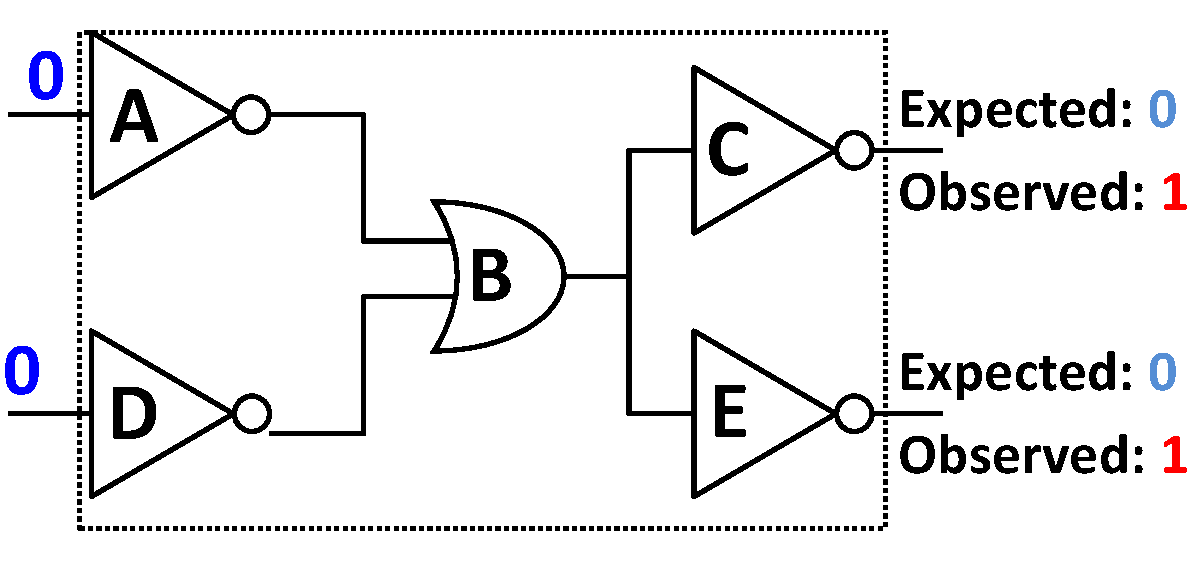
\includegraphics[width=0.6\columnwidth]{mbd-example.pdf}
	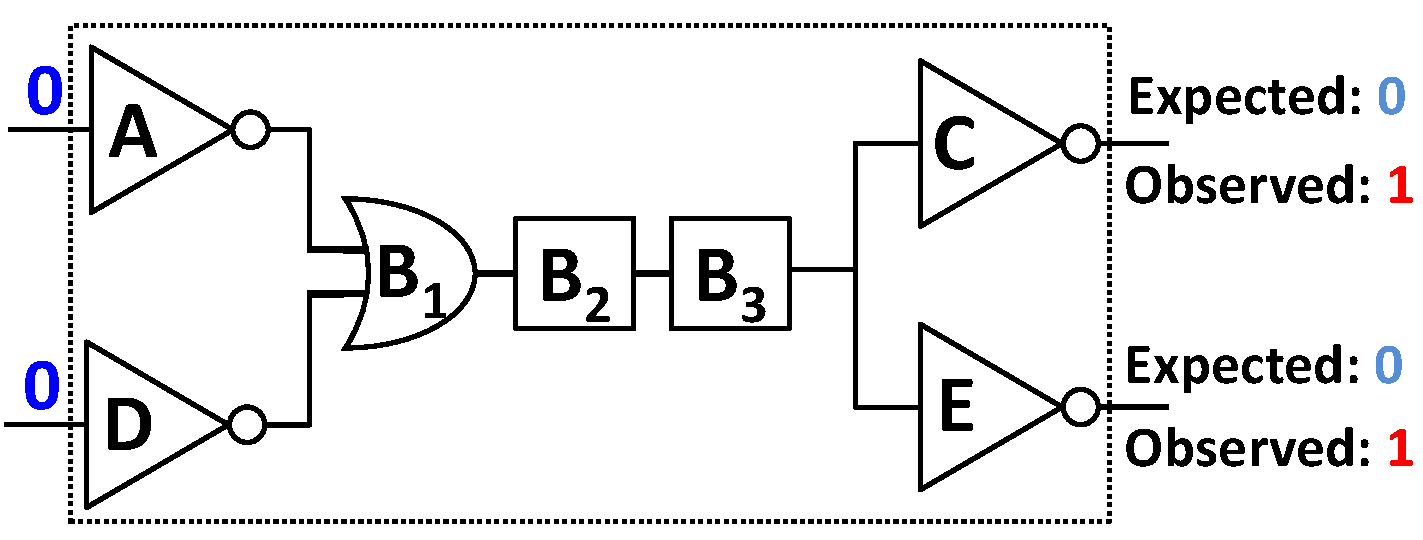
\includegraphics[width=0.5\textwidth]{mbd-example_cropped.pdf}
%    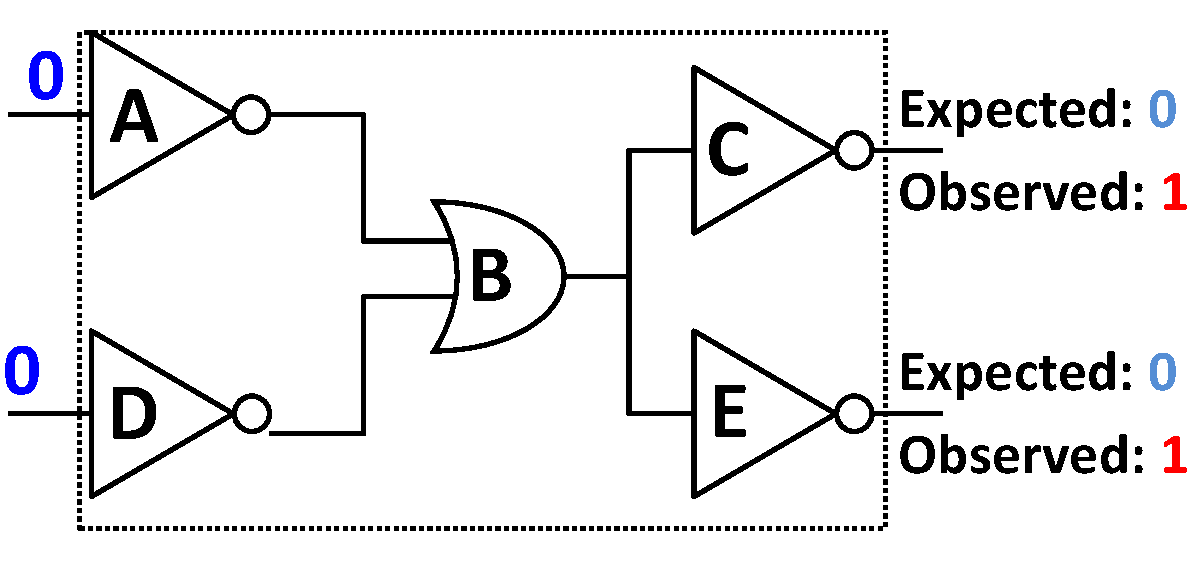
\includegraphics[width=0.75\textwidth]{mbd-example}
    \caption{A simple example of a DX problem with multiple consistent diagnoses}
    \label{fig:mbd-example}
\end{figure}

% The problem: too much diagnoses
\subsubsection{MBD with Data-Driven Prioritization} 
% Focus on cases where the model is correct 
First, we investigate how MBD and DDD can be integrated in scenarios where an accurate (but possibly incomplete) model of the diagnosed system is available together with past observations. 
% MBD are often consistency-based. These have a lot of diagnoses
Most MBD algorithms are consistency-based, in the sense that they aim to return every diagnosis  that is consistent with the system model and observations. 
Unfortunately, there can be many consistent diagnoses for a given set of observations, thus providing poor fault isolation~\cite{stern2015many}. 
For example, Figure~\ref{fig:mbd-example} shows a simple DX problem where the diagnosed system is a small Boolean circuit. Components $A$, $D$, $C$, and $E$ are NOT gates, component $B_1$ is an OR gate, and components $B_2$ and $B_3$ are buffer gates (which are supposed to output the same value as their input). One possible diagnosis is that component $B_1$ is faulty, and has output zero instead of one. Similarly, either component $B_2$ or $B_3$ may be faulty, 
and there are also possible double fault diagnoses (i.e., diagnoses that assume two components are faulty): $\{ A,D \}$ and $\{C,E\}$. It is difficult to assess which of these five diagnoses is correct or more likely. 
As shown in PI Stern's prior work, even if we only focus on minimal cardinality diagnoses (those with the smallest number of assumed faulty components) the number of possible diagnoses can be very large, even in standard MBD benchmarks~\cite{stern2015many}. Thus, MBD algorithms require some way to prioritize their results diagnoses. We propose a data-driven approach to do so, as follows. 


% The solution: Bayesian reasoning. But that needs priors - DDD to save the day!!!
First, we will use ML algorithms to learn a set of classifiers, one per component, such that each classifier aims to detect whether its component is healthy or faulty given observations about the system's behavior. 
Then, these classifiers are used with the current observations ($OBS$) to produce a classification (healthy/faulty) for each component. Importantly, most classifiers also provide a {\em confidence} measure, which estimates the likelihood that the classification is correct. These confidence scores are used 
to better prioritize the consistent diagnoses returned by MBD algorithms, e.g., as priors in a Bayesian likelihood computation~\cite{abreu2009new}. Moreover, these data-driven confidence scores can also be used as a heuristic to speed up the search for consistent diagnoses. This data-and-model driven approach is very general, and our initial results on software  diagnosis show promise~\cite{elmishali2016dataAugmented}. 

%as priors when computing the likelihood of a-priori probability that such learned functions to prioritize the consistent diagnoses. The resulting algorithm will be a combination of MBD algorithms for generating diagnoses and DDD algorithms to prioritize them. This hybrid data-and-model driven approach for MBD is very general, and our initial results on software diagnosis~\cite{elmishali2016dataAugmented} show promise. 


 
%function that classifies components as healthy or faulty given $OBS$. % and various model properties. 
% Classifiers learned by machine learning algorithms often also provide some confidence measure, which estimates the likelihood that the classification is correct. 
%We propose to use such learned functions to prioritize the consistent diagnoses. The resulting algorithm will be a combination of MBD algorithms for generating diagnoses and DDD algorithms to prioritize them. This hybrid data-and-model driven approach for MBD is very general, and our initial results on software diagnosis~\cite{elmishali2016dataAugmented} show promise. 
%Then, the confidence score of each component as the a-priori probability that such learned functions to prioritize the consistent diagnoses. The resulting algorithm will be a combination of MBD algorithms for generating diagnoses and DDD algorithms to prioritize them. This hybrid data-and-model driven approach for MBD is very general, and our initial results on software diagnosis~\cite{elmishali2016dataAugmented} show promise. 



% Future challenges
\begin{problem}
Formalize this data-and-model driven prioritization approach and demonstrate its usefulness on a range of domains. 
\end{problem}
We will also study the relationship between the number of past observations we have, the size and structure of the analyzed system, and the expected usefulness of this data-augmented approach over the data-agnostic MBD approach: 
\begin{problem}
Analyze the trade-off between number of available observations and the quality of data-and-model driven diagnoses.
\end{problem}
Since in many cases most past observations are of a healthy scenario and only a few faulty scenarios are available, we will study how to build DDD models that can use mostly healthy scenarios and still help in prioritizing diagnoses. We will also seek to guide the MBD algorithm with knowledge from the DDD model, e.g., providing a more informed heuristic to heuristic-search-based MBD algorithms, such as HA*~\cite{feldman2006two} and CDA*~\cite{williams2007conflict}. %, can guide their search towards adding earlier components that are more likely to be part of the diagnoses according to the DDD model. 


%\note{I feel that we need more here. Maybe something about uncovering the theory behind this combination of data and model?}
%\subsubsection{Learning Plausible Diagnoses} 
%\subsubsection{Faster Diagnosis Using Data} %% Maybe this is a more accurate title for what we are proposing?
%\note{This is a good candidate for cutting or folding into the previous section.}
%Observing past nominal and faulty behavior can also be used to speed up the diagnostic process. In particular, we propose to learn from observations special cases which are easy to diagnose. Indeed, it is well-known in the MBD literature that some types of system models are  easy to diagnose. Also, several techniques have been proposed to compile a given system model to an easy-to-diagnose model such as Decomposable Negation Normal Form~\cite{darwiche2001decomposable} and Ordered Binary Decision Diagrams (OBDDs)~\cite{torta2006onTheUse}. These compilation methods, however, sometimes result in a model that is exponentially larger than the original system model. 

%We propose a general approach that makes use of past observations to diagnose easy instances, based on PI Juba's recent work~\cite{juba2016aaai}.  The main idea is to search the space of simple candidate diagnoses (e.g., $k$-DNFs) over past observations, that are approximately the most likely possible easily verified diagnoses of a certain faulty behavior. 

%that one can learn a model to diagnose them. This circumvents the general problem of learning a DDD model, while provides fast and effective solutions to a meaningful subset of the cases.While the theory of this approach has been outlined by PI Juba's prior work~\cite{juba2016aaai}, no empirical support for the usefulness of this theory was given. In the proposed research we will evaluate its usefulness on standard diagnosis benchmarks (see Section~\ref{sec:evaluation}). 


%In addition, it is not fully specified how to identify when finding a diagnosis is easy. 
%% I'm not sure what the above means.Moreover, as the diagnosed system becomes more complex, searching the space of possible conditions will become intractable, thus suggesting more intelligent search techniques are needed. We will meet and address these challenges in the proposed research.  

%it will be more difficult to search the space of conditions as well as to identify
%Moreover, the model being learnt
%\note{Roni: we should add here more challenges, along the lines of the type of models we can learn, the type of special case, the sample complexity of all this, the overall integration with MBD on top of this, etc.}



%Learn conditions on sensors taht yield a small set of possbile diagnoses (see AAAI paper)

\subsubsection{PAC Semantics for Model-based Diagnosis}
%\note{Warning: drafts below!}


% In MBD we're used to incomplete models, but the approximate models are harder for us. But still, we rock at reasoning, so what should we do?
%Since modeling is known to be very difficult in model-based diagnosis, much of the MBD literature has dealt with weak types of models. One such well-studied weak type of model is the {\em weak fault model} (WFM), in which only the nominal behavior of the components is modeled while there is no knowledge of how components behave when they are faulty. However, even such a weak fault model is usually very difficult to obtain. Indeed, predicting {\em exactly} how components will {\em always} behave in a complex system is very difficult. In particular, obtaining component behavior rules that are always correct is very hard, and learning such rules is practically impossible in most cases.
Predicting {\em exactly} how components will {\em always} behave in a complex system is very difficult. In particular, obtaining component behavior rules that are always correct is very hard, and learning such rules is practically impossible in many cases. However, it may be possible to learn component behavior rules that are {\em probably} correct in {\em most cases}. Specifically, we aim to learn and reason about PAC-semantic rules that describe the relationship between 
the health of subset of components and their functionality. 
A simple example of such component behavior rules is Horn clauses such as $h(A)\rightarrow (o = i_1 \wedge i2)$
where $A$ is a component in the system, $h(A)$ is a predicate denoting that $A$ is healthy, and $i_1$, $i_2$, $o$ are the input and output values of $A$, respectively. Such rules are commonly used in MBD algorithms,
but in PAC semantics each rule is also associated with the probability that it is false (the error function). 

%This is exactly w
%We propose to leverage the power of PAC semantics to enable  reasoning about behavior rules that are learned from data, and are thus only probably correct. 
%Specifically, we aim to learn and reason about rules that describe the relation between  the health of subset of components and their functionality. 
%but the novelty is the error function that is added when using PAC semantics, associating each rule with the probability that it is false. 

%There is also a line of work on {\em robust fault detection and isolation} (robust FDI)~\cite{chen2012robust,frank1997survey} that is specifically designed to develop fault detection and diagnosis algorithm that are robust to inaccuracies in the system model. Most work on robust FDI do not apply logic-based reasoning and instead attempt to model the possible ways in which the model can be inaccurate. This is orthogonal to our approach, where we do not assume such a-priori knowledge about the inaccuracy of the model.  


\paragraph{Learning PAC-Semantic Rules for MBD.}
% To learn PAC rules we need probes
Learning PAC-semantic rules requires some data about the values of components' inputs and outputs 
during past observations. Observing such values is known in the DX literature as ``probing''~\cite{deKleer1987diagnosing,rish2004real,feldman2010model}. 
Ideally, all the input values and output values of all components in all past observations are available, 
and are then used to learn behavior rules for each component. 
Probes, however, can be costly to deploy and monitor and thus we expect to have probes only in some of the observations and over a subset of the components. 

% Also, we will learn not specific horn-clauses but something more general
To simplify the learning task and to be able to obtain more information from past observations, we intend to learn and reason about rules that are more complex than simple Horn clauses. This includes rules where the left hand side consists  of more than a single component,  e.g., $(h(A)\wedge h(B)) \rightarrow o\equiv i_1\wedge i_2$, where $B$ is another component, 
and rules that include both health predicates and sensor values in their left-hand side are also possible, e.g., 
$(in_1=1 \wedge h(A) \wedge h(B))\rightarrow o\equiv 1$. Such rules are expected to be easier to learn from data, as they may require less detailed knowledge about the internals of the diagnosed system. 
%Finally, rules that include both health predicates and sensor values in their left-hand side are also possible, e.g.,  $(in_1=1 \wedge h(A) \wedge h(B))\rightarrow o\equiv 1$. 
%Existing MBD algorithms are capable of reasoning with all these types of rules to obtain consistent diagnoses, but, of course, the resulting diagnoses can be less accurate. 
However, as the left-hand side of these rules grows, we expect the resulting diagnoses to be less accurate. 
Similar to learning PAC-semantic rules for planning, here too there can be a difference between the rules we can learn and the rules we should learn. This is because learning more rules will result in finding more accurate diagnoses but at the cost of greater complexity. 
\begin{problem}
Analyze the trade-off between diagnostic accuracy and complexity. 
\end{problem}


[[Two approaches: direct ``supervised'' learning to identify a healthy behavior, and implicit learning, where we avoid learning specific rules from the data, but rather try to learn proofs about the current observation that we want to classify]]

%introduces a trandel The latter challenge embodies a trade-off between  diagnostic accuracy and complexity: more rules may allow finding more accurate diagnoses but at the cost of greater complexity. 

%the inputs and outputs of internal 
%Such observations can be available in system, by using {\em probes}.  However, probes can be costly to deploy and monitor, and thus we do not expect to have probes over all components and in all observations. \note{Not done yet - will continue in 3 hours} for MBD raises fundamental challenges we aim to address: (1) how to identify rules that describe an individual component's behavior  and (2) how to choose which rules to learn. 

\paragraph{MBD with PAC-Semantic Rules}
% Statement of operation: we will reason about rules that are only sometimes true
%PAC semantics are especially suitable for model-and-data driven methods, since 
Given a system description that consists of a set of PAC-semantic rules, there is still the challenge 
of how to perform effective diagnostic reasoning with such rules. 
%A key objective in the proposed research is to study exactly this and develop MBD algorithms that are able to reason with rules using PAC semantics. 
Existing MBD algorithms are capable of reasoning about incomplete models (a classical example is the weak fault model assumption). However, most MBD algorithms do not reason about the likelihood that the rules they use for reasoning -- i.e., the system model -- may be incorrect. 
% The problem 
Concretely, the diagnostic challenge is to find the most likely diagnosis (or a set of highly likely diagnoses) given a set of rules that describe various relations between observed system behavior and components' health, such that each rule is associated with a probability that it is true, referred to as the rule's {\em validity}. 
% Why it is not trivial
A simple approach can be to limit the diagnosis algorithm to only use rules whose validity is over some given value. This approach has several drawbacks. First, there is no principled way to set this threshold. Second, this approach can result in sub-optimal results, as follows. 
Assume that we have 3 rules $r_1$, $r_2$, and $r_3$ such that the probabilities that each rule is correct are 0.8, 0.8, and 0.7, respectively. 
Now, imagine that there are two diagnoses $\omega_1$ and $\omega_2$, such that $\omega_1$ is derived by reasoning about $r_1$ and $r_2$, while $\omega_2$ is derived by reasoning only about $r_3$. Which diagnosis is more likely? 
If we assume that rules' likelihoods are independent, than clearly $\omega_2$ is more likely. But, if we set the rules' threshold to 0.75, our diagnosis algorithm will not find $\omega_2$. 

% We will solve it!
Thus, when diagnosing with PAC-semantic rules,  the likelihood of a diagnosis is affected by  the validity of the rules used to infer it, as well as any other prior knowledge about the components' failure likelihood (such as the learned priors discussed in earlier in this proposal). We will develop algorithms that take these probabilities into account:
\begin{problem}
Develop diagnosis algorithms based on heuristic search that search for the most likely diagnoses in this setting, as well as appropriate heuristics.
\end{problem}
% Diagnosis for physical systems
Above, we have implicitly assumed that logical rules can be learned to approximately represent the system. However, systems may be too complex to be represented by simple logical rules. In such cases, we may also learn rules that {\em approximate} some parts of the system behavior. While learning a complete model of a physical system is bound to be futile, we will aim for learning cases that are common enough and can be approximated by a learned function. A preliminary framework for how to do so was recently outlined by PI Juba~\cite{juba2016aaai,juba2016conditional}.




% Wrapping it up -- a complete learning and diagnosing framework that exploits the benefits of PAC semantics and lay on sound theoretical ground
%As in planning, the merit of developing diagnosis algorithm able to reason with PAC semantic rules is especially important to demonstrate the ability to perform a complex reasoning task like diagnosis without a complete system model and based on the theoretical grounds of PAC semantics. 


\subsection{Evaluation}
\label{sec:evaluation}

%Beyond developing the theoretical understanding of the roles of models and observations in planning and in diagnosis, an important outcome of the proposed research is applicable planning algorithms and diagnosis algorithms that can outperform the state-of-the-art. This objective is feasible as we will exploit both model and observations, while most planning algorithms and diagnosis algorithms are not designed to take both into account. 
The developed algorithms will be compared against the state-of-the-art on standard benchmarks. In planning, 
we will focus on the FastDownward planning system~\cite{helmert2006fast} and problems from the international planning competition (IPC). 
%we will focus on domain-independent planning algorithms such as those given in the FastDownward planning system~\cite{helmert2006fast}. 
In addition, we will also experiment on domain-specific planning problems such as the multi-agent planning problems that have been deeply studied by PI Stern~\cite{sharon2013increasing,sharon2015conflict,boyarski2015icbs,boyrasky2015dont,maliah2016collaborative}. 
For the incomplete model setting, we will introduce ``noise'' or mask part of the model in the benchmarks described above. Then, we will compare against model-based methods that only reason about the noisy model, and data-driven methods that ignore the available partial model. 
Another application that we intend to aim for is robotics. 
[[Roni: new addition]]
Robotics is an important application for planning, in which the challenge of not having an exact domain/environment model is common. Evaluating our algorithms on physical robots is beyond the scope of this project, but there are accepted simulators such as Gazebo and Stage which we intend to use. To this end we will build on and extend the Search-Based Planning Library (SBPL)~\cite{likhachev2014sbpl}, that has easy integration with such simulators and real robots. 

For DX, we will focus on Boolean circuits from the international DX competition~\cite{poll2011third}, introducing ``noise'' to make the model incomplete, if needed. In addition we will experiment on diagnosing software systems, using real open source software projects, such as the data used in PI Stern's prior work~\cite{Zamir2014UsingMD,elmishali2016dataAugmented,barIlan2017learningSoftwareBehavior}. 

%Similarly, we will evaluate the developed MBD algorithms over standard MBD benchmarks such as Boolean circuits~\cite{hansen1999unveiling,brglez1999design}. An additional domain we will experiment on is software diagnoses, where we will experiment on data from open source projects, such as the data used by Elmishali et al.~\cite{elmishali2016dataAugmented}. 




%To evaluate the developed planning algorithms, we will compare them against state-of-the-art domain-independent planning algorithms over standard planning benchmarks, such as those given in the FastDownward planning system~\cite{helmert2006fast} (available at \url{http://www.fast-downward.org}). In addition, we will also experiment on domain-specific planning problems such as the multi-agent path finding problem, which has been deeply studied by PI Stern~\cite{sharon2013increasing,sharon2015conflict,boyarski2015icbs,boyrasky2015dont}. Similarly, we will evaluate the developed MBD algorithms over standard MBD benchmarks such as Boolean circuits~\cite{hansen1999unveiling,brglez1999design}. An additional domain we will experiment on is software diagnoses, where we will experiment on data from open source projects, such as the data used by Elmishali et al.~\cite{elmishali2016dataAugmented}. 

 %attempt to directly answer the quetion (not sure this fits for planning, but it does for diagnosis and plan recognition), data-driven methods that learn an model and then apply reasoning, and then some new methods by us that integrate all these things nicely. 


%4. From BSF guidelines: Risk analysis and alternative paths that will be followed if the suggested research plan fails (only in those fields in which it is relevant);
%\section{Risk Analysis and Alternative Plans}
%\note{Maybe we want to avoid this section, even though it is in the guidelines}
\vspace{-0.35cm}
\section{Collaboration between the Principal Investigators}
The PIs began scientific discussions on some of the topics discussed in this proposal while they were post-doctoral fellows at Harvard University.
%PI Juba and PI Stern met when they were both post-doctoral fellows at Harvard University. 
%While PI Juba and PI Stern study very different aspects of Artificial Intelligence, during that time they had many scientific discussions on some of the topics discussed in this proposal. However, PI Stern soon returned to Israel for a faculty position at BGU, before these discussions could mature into a fruitful scientific collaboration. 
%Throughout the years, the PIs have met in general AI conferences and 
Their research interests have recently aligned further, 
with the recent work of PI Juba on the theoretical foundations of learning for planning and abductive reasoning, and the years of experience of PI Stern in developing planning and diagnosis (a form of abductive reasoning) algorithms. 
Both PIs are young researchers and hope to develop this joint interest to a long-term collaboration on the fundamental topics outlined in this proposal.
%, but funding is needed to support it.  
[[Roni: add here preliminary work]]
As part of working on this proposal, the PIs have co-authored two research papers. The first was published in the International Joint Conference of Artificial Intelligence (IJCAI) in  2017~\cite{stern2017efficientAndSafe}, and the second was submitted to the AAAI 2018 conference and is currently under review. These papers provide initial steps for portions of this proposal: the first is on learning an action model that is sufficient to find a sound plan, and the second is on learning a system model that is sufficient to find faulty components in a diagnosis setting. Both works are preliminary in that they assume a very limited type of planning and diagnosis and include no experimental evaluation. The proposed research project will allow the PIs to continue  work in these directions.


The planned mechanisms to facilitate the collaboration include holding an annual meeting at either BGU or WUSTL, as well as having students from each group travel to the other group. In between these annual face-to-face meetings, the collaboration will be continued via regular Skype meetings. The PIs have carried out their collaboration thus far with such Skype meetings which has led to a series of preliminary results (e.g.,~\cite{stern2017efficientAndSafe}). 
[[Further concrete coordination mechanisms? Serve on students' committees remotely?]]


%[Avi, Michal, Iliya, Barak, Amir, Orel, Hila, Ester, Netanel, Gal, Dor, Daniel, Yossi, ]


\section{Broader Impacts}
Automated planning has numerous applications beyond academia, e.g., in the development of autonomous vehicles and other robots. Similarly, automated diagnosis also has obvious applications, e.g., in the maintenance of complex systems and their software. Indeed, we intend to evaluate our diagnosis algorithms in particular on such engineering problems. %and problems a. 
We expect the algorithms that we develop for planning and for diagnosis to improve the speed, quality, and breadth of applicability of these algorithms. 

The PAC search framework we will develop will open up the field of heuristic search to the notion of probabilistic guarantees, which will allow search algorithms in general to scale to much larger problems while still preserving a useful notion of solution quality. 

Also, our methods for integrating models and data may carry over to other tasks such as coordination of multi-agent systems and scheduling with their own real-world applications. By studying and understanding the effect of having a partial model on the theoretical limits of what can be learned from data, one can decide the cost-effectiveness of generating such a model. 
This is especially important since modeling the world is notoriously difficult, and choosing what not to model is a key problem in practical applications of AI. 

Finally, most funds are requested to support graduate students, reflecting our focus on education and our commitment to training the next generation of researchers. 

\section{Results from prior NSF support}
PI Juba supervised two REU students supported by IIS award \#1560191 (``Big data analytics REU site'') during summer 2016, and another student during summer 2017. The first two students worked on finding human-understandable descriptions of anomalous webcam images by using meta-data for the images. {\em Intellectual Merit:} Previous works on ``explaining anomalies'' did not not provide such cross-modal explanations, and often only operated on a per-example basis, as opposed to summarizing characteristic features of groups of anomalies as in our work. The third student helped develop and analyze an algorithm for the conditional linear regression problem, identifying a $k$-DNF event of near-optimal probability on which a good regression fit exists. {\em Intellectual Merit:} Previous algorithms either ran in time exponential in the sparsity of the regression fit or could only recover a polynomially small fraction of the ideal event. {\em Broader Impacts:} These REU students (two female) were trained in research, and publications describing our results are respectively under review~\cite{qi2018} and in preparation~\cite{calderon2018}. The work concerned the development and use of principled algorithms to produce human-understandable rules that we expect will be useful for data analysis tasks outside academia. Dr. Juba also recently received CCF award \#1718380, but this support just began in September 2017. The project concerns developing the use of ``sum-of-squares'' proofs for probabilistic reasoning. {\em Intellectual Merit:} sum-of-squares has been used to design approximation algorithms by taking a ``Bayesian'' perspective on optimization, but surprisingly it had not been used as a tool for probabilistic inference to date. It features tractable solvers and supports a rich family of probabilistic inferences. {\em Broader Impacts:} The work will support the training of graduate student and the development of probabilistic reasoning techniques that have applications in broad areas of AI. In turn, these techniques should have applications as part of AI systems deployed in the real world.

\pagebreak
\bibliographystyle{plain}
\bibliography{references}

\newpage
%5. From BSF guidelines: An account of available U.S. and Israeli resources, including all personnel and equipment relevant to the research;

\section*{Facilities, Equipment, and Other Resources}
%\section*{Available U.S. and Israeli Resources}
%NOTE: This section does not need to appear in the 15pg Project Description. NSF permits a separate section to account for Facilities and Equipment, etc. Hence I've moved it to the position it will appear in the final document, after the references.

One Ph.D. student and one Master’s student from PI Stern's group, which currently includes three Ph.D. and ten Master's students, will participate in the proposed research. One Ph.D. student from PI Juba's lab will work on this project, and a second Ph.D. student will be recruited during the project starting in the second year.
%\note{Roni: Brendan, please fill in your estimate of how many people will work on the project. From our discussion on budget I think you aim for one student, right?}

The facilities available at BGU for PI Stern's
lab will be available for this research, including basic office facilities and a server for performing heavy duty computations. PI Juba's lab will have access to the ``Machine Learning Cluster,'' a  shared cluster of five machines, each with 12--16 cores and at least 128GB RAM. (Some also feature GPUs.) WUSTL will also provide office space and access to libraries and electronic resources to PI Juba's group. BGU and WUSTL will provide the facilities for holding the annual research meetings. 

\newpage
\section*{Data management plan}
We plan to publicly share the source code for the implementations of the algorithms developed in this project ``as-is'' on Bitbucket (\url{https://bitbucket.org}) under the MIT License (\url{http://opensource.org/licenses/MIT}), a standard, permissive open source license. In this way, we plan to release the code developed for the project within six months of publication.

Most of our evaluation will be performed using standard benchmarks, or benchmark instances already collected for another project; we do not anticipate compiling substantial new data sets as part of this work. However, in some cases we will generate synthetic data sets, and in these cases we will make the code for generating the synthetic data available along with the source code for the evaluated system. 

\end{document}

